Duidelijk duiden dat dit hoofdstuk gebaseerd is op de paper van stefanos en bajoumi.
Biological transporter. This chapter will discuss the function + operation +
computational analysis with beadspring model and LAMMPS

\section{Rotaxane Formation}


talk about the constituents. Neutravidin, nanopore, DNA -> toehook.

Formation due to changin of the voltage. Measure current and infer the state of the
complex.





\begin{figure}[ht]
  \begin{centering}
  \adjustbox{minipage=1.3em,valign=t}{\subcaption{}\label{sfig:testa}}%
  \begin{subfigure}[t]{\dimexpr.8\linewidth-1.3em\relax}
  \centering
  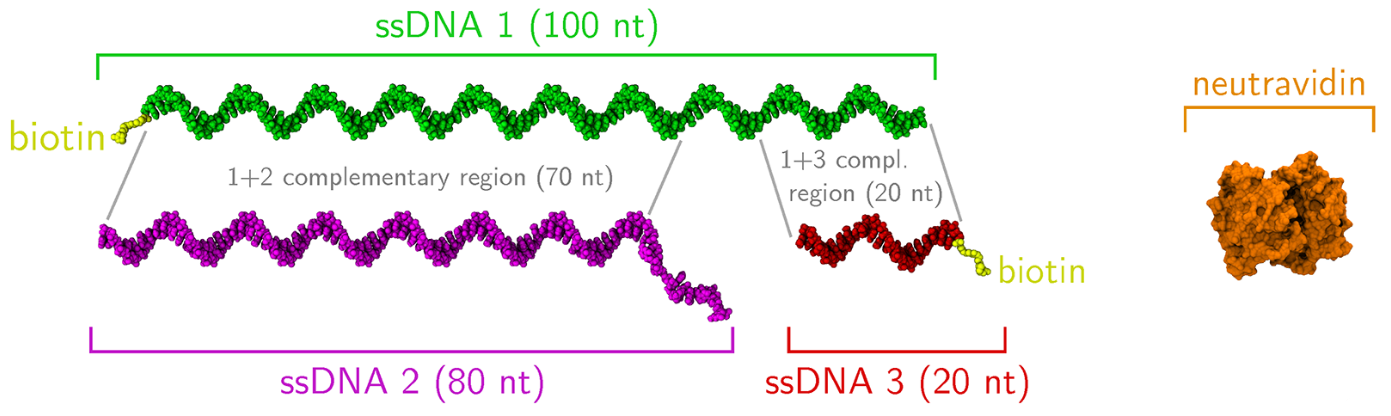
\includegraphics[width=\linewidth,valign=t]{Figures/RConstruction1.png}
  \end{subfigure}%
  \vspace{0.5cm}
  \adjustbox{minipage=1.3em,valign=t}{\subcaption{}\label{sfig:testa}}%
  \begin{subfigure}[t]{\dimexpr.8\linewidth-1.3em\relax}
  \centering
  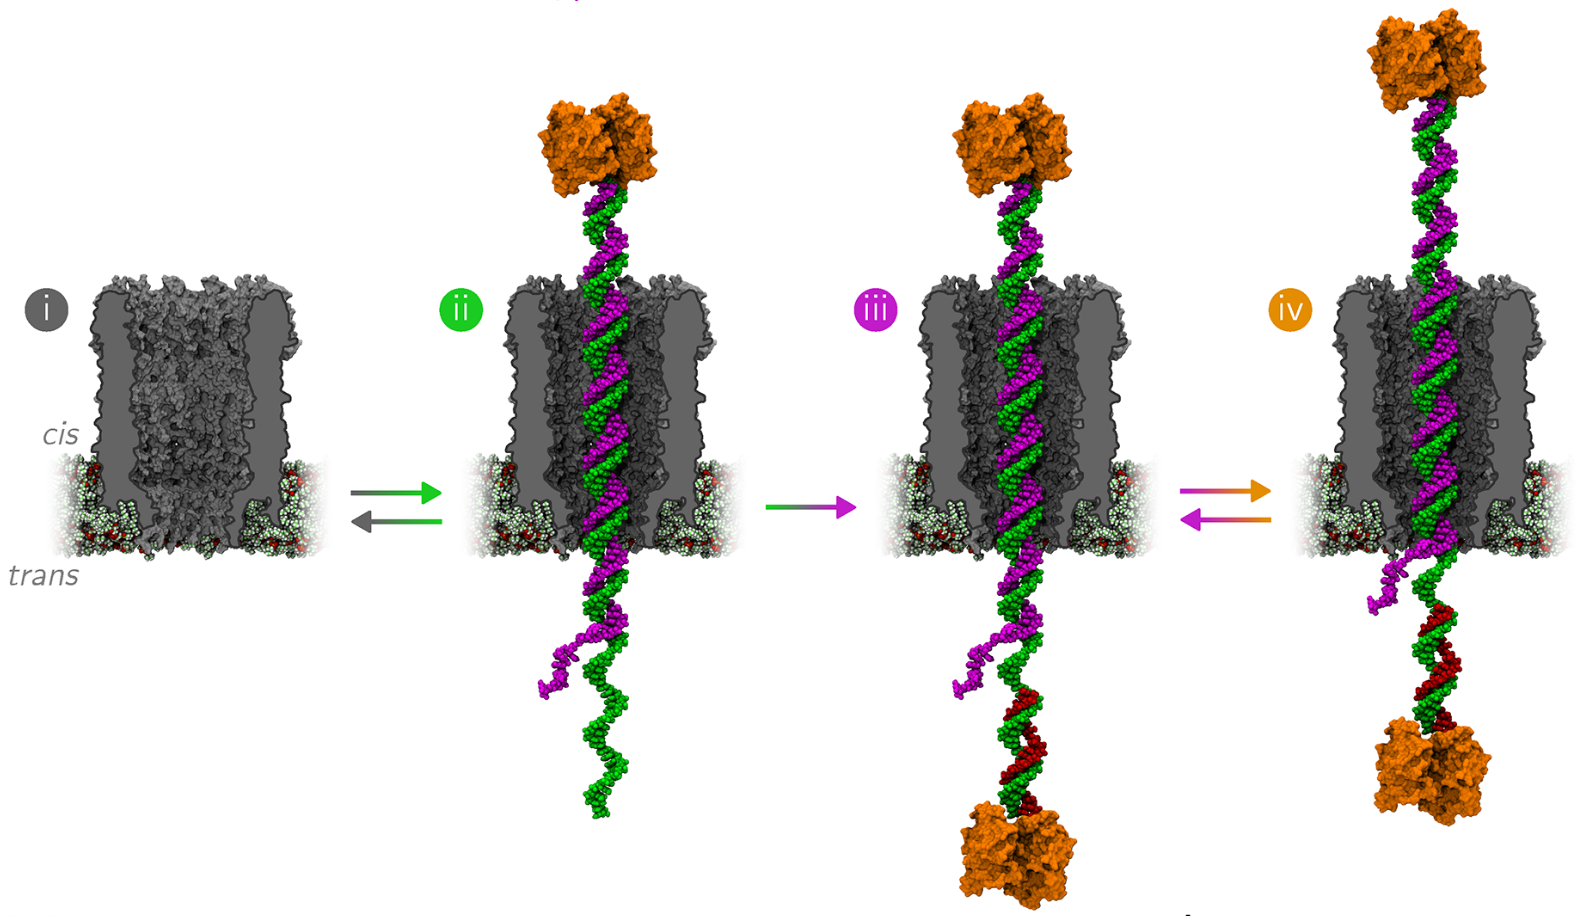
\includegraphics[width=\linewidth,valign=t]{Figures/RConstruction2.png}
  \end{subfigure}%
  \vspace{0.5cm}
  \adjustbox{minipage=1.3em,valign=t}{\subcaption{}\label{sfig:testb}}%
  \begin{subfigure}[t]{\dimexpr.8\linewidth-1.3em\relax}
  \centering
  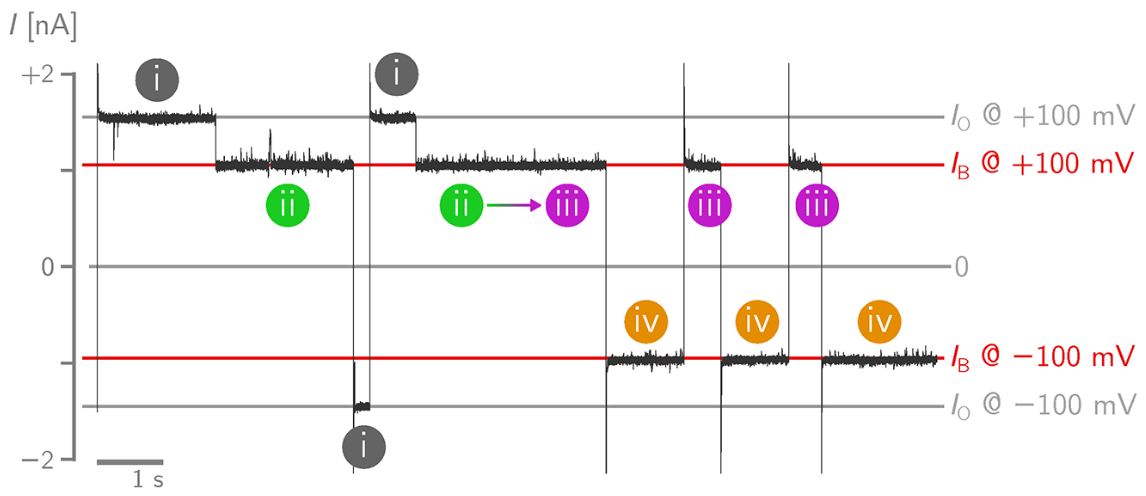
\includegraphics[width=\linewidth,valign=t]{Figures/RConstruction3.png}
  \end{subfigure}
  \caption{This is a figure [.]}
  \label{fig:test}
  \end{centering}
\end{figure}
